\documentclass[
  a4paper,
  oneside,
  % 12pt
]{report}

% Configura as margens das páginas
\usepackage[
  top    = 3cm,
  bottom = 2.25cm,
  left   = 2cm,
  right  = 2cm
]{geometry}

\usepackage{babel}
\usepackage{enumitem}
\usepackage{amsmath}
\usepackage{booktabs}
\usepackage{bm}
\usepackage{float}
\usepackage{circuitikz}
\usepackage{siunitx}
\usepackage{steinmetz}
\usepackage{amssymb}
\usepackage{setspace}
\usepackage{subcaption}
\usepackage{listings}
\usepackage{courier}
\usepackage{xcolor}
\usepackage{fancyhdr} % Para cabeçalhos e rodapés personalizados

% Possibilita hiperlinks no texto
\usepackage[pdftex,
  % backref,
  linktocpage = false,
  colorlinks  = true,
  linkcolor   = black,
  anchorcolor = blue,
  citecolor   = blue,
  urlcolor    = blue
]{hyperref}


% Configuração do fancyhdr
\pagestyle{fancy} % Estilo de página fancy
\fancyhf{} % Limpa todos os cabeçalhos e rodapés atuais
\renewcommand{\headrulewidth}{0.4pt} % Espessura da linha do cabeçalho
\renewcommand{\footrulewidth}{0.4pt} % Espessura da linha do rodapé

% Cabeçalho (header)
\fancyhead[L]{\leftmark} % Coloca o nome da seção atual à esquerda
\fancyhead[R]{\thepage} % Número da página à direita

% Rodapé (footer)
\fancyfoot[L]{} % Texto esquerdo no rodapé
\fancyfoot[R]{} % Texto direito no rodapé

% Configuração do pacote listings
\renewcommand{\lstlistingname}{Código}
\lstset{
  language=Python,
  tabsize=2,
  basicstyle=\small\ttfamily,
  keywordstyle=\bfseries\color{blue!40!black},
  commentstyle=\color{gray}\itshape,
  numbers=left,
  numberstyle=\tiny,
  breaklines=true,
  captionpos=b,
  xrightmargin=0pt,
  xleftmargin=15pt,
  literate={á}{{\'a}}1 {à}{{\`a}}1 {â}{{\^a}}1 {ã}{{\~a}}1 {é}{{\'e}}1 {ê}{{\^e}}1 {ë}{{\"e}}1 {í}{{\'i}}1 {ç}{{\c{c}}}1 {Ç}{{\c{C}}}1 {õ}{{\~o}}1 {ó}{{\'o}}1 {ô}{{\^o}}1 {ú}{{\'u}}1 {δ}{{\ensuremath{\delta}}}1 {Ξ}{{\ensuremath{\Xi}}}1 {Ψ}{{\ensuremath{\Psi}}}1 {Γ}{{\ensuremath{\Gamma}}}1 {λ}{{\ensuremath{\lambda}}}1 {θ}{{\ensuremath{\theta}}}1 {┌}{{\char192}}1
  {│}{{\char179}}1
  {┐}{{\char191}}1
  {└}{{\char218}}1,
}

\setstretch{1.5} % Espaçamento de 1.5 entre linhas

% Comandos personalizados
\newcommand{\phasor}[2]{#1 \,\phase{\,#2^\circ}} % Comando para fasor
\newcommand{\txt}[1]{\;\mathrm{#1}} % Comando para texto em modo matemático

\NewDocumentCommand{\voltage}{m o}{%
  \IfValueTF{#2}
    {#1 \,\, \text{#2V}}
    {#1 \,\, \text{V}}%
}

\NewDocumentCommand{\apparentpower}{m o}{%
  \IfValueTF{#2}
    {#1 \,\, \text{#2VA}}
    {#1 \,\, \text{kVA}}%
}

% Contador para exercícios
\newcounter{exercise}
\newcommand{\exercise}{%
  \stepcounter{exercise}
  \section*{Exercício \arabic{exercise}}
}

% Ambiente de resolução
\setlength{\parindent}{0pt} % Remover indentação dos parágrafos

\everymath{\displaystyle}

\begin{document}

% \input{pre-textual/cover.tex} % Capa do documento
\section{Takagi-Sugeno Fuzzy Model}

The design procedure begins with representing a given non-linear plant by the Takagi-Sugeno fuzzy model. This model is characterized by fuzzy IF-THEN rules which describe local linear input-output relations of a non-linear system. The TS Fuzzy model expresses the local dynamics of each fuzzy rule using a linear system model, while the global model is achieved by combining these linear system models 

The $i$-th fuzzy rules for Continuous Fuzzy Systems (CFS) are of the following forms:

\begin{enumerate}
  \item[] \textit{\textbf{Model Rule i:}}
  \begin{itemize}
      \item[] \textbf{IF} $z_1(t) \txt{is} M_{i1} \txt{and} \dots \txt{and} z_p(t) \txt{is} M_{ip}$
      \item[] \textbf{THEN} $\begin{cases}
        \dot x = A_i x(t) + B_i u(t) \\
        y = C_i x,
      \end{cases}, \hspace{12pt} i = 1, 2, \dots, r.$
  \end{itemize}
\end{enumerate}

Here, $M_{ij}$ is the fuzzy set and $r$ is the number of model rules; $x(t) \in \mathbb{R}^n$ is the state vector, $u(t) \in \mathbb{R}^m$ is the input vector, $y(y) \in \mathbb{R}^q$ is the output vector, $A_i \in \mathbb{R}^{n\times n}$, $B_i \in \mathbb{R}^{n\times m}$ and $C_i \in \mathbb{R}^{q\times n}$; $z_i(t), \dots, z_p(t)$ are known premise variables which may be functions of the state variables, external disturbances, and/or time.

Given a pair of $(x(t), u(t))$, the final outputs of the CFS are inferred as follows:

\begin{equation}
  \dot x = \frac{\sum\limits_{i=1}^{r} w_i(z(t))\{A_i x(t) + B_i u(t)\}}
  {\sum\limits_{i=1}^{r} w_i(z(t))} =
  \sum\limits_{i=1}^{r} h_i(z(t))\{A_i x(t) + B_i u(t)\}
\end{equation}

\begin{equation}
  y(t) = \frac{\sum\limits_{i=1}^{r} w_i(z(t)) C_i x(t)}
  {\sum\limits_{i=1}^{r} w_i(z(t))} =
  \sum\limits_{i=1}^{r} h_i(z(t))C_i x(t)
\end{equation}

where $z(t) = \left[z_1(t), z_2(t), \dots, z_p(t)\right]$, 

\begin{align}
  w_i(z(t)) &= \prod\limits_{j=1}^{p} M_{ij}(z_j(t)) &\txt{and}&&
  h_i(z(t)) &=  \frac{w_i(z(t))}{\sum\limits_{j=1}^{r} w_{i}(z(t))},
\end{align}

for all time $t$. The term $M_{ij}(z(t))$ is the grade of membership of $z_j(t)$ in $M_{ij}$. Since
\begin{equation}
\sum_{i=1}^{r} w_i(z(t)) > 0, \quad w_i(z(t)) \geq 0, \quad i = 1, 2, \dots, r,
\end{equation}
we have
\begin{equation}
\sum_{i=1}^{r} h_i(z(t)) > 0, \quad h_i(z(t)) \geq 0, \quad i = 1, 2, \dots, r.
\end{equation}
\chapter{DC-DC Converters Modeling}

\section{Buck Converter}

The buck converter circuit is illustrated in \autoref{fig:buck_converter}. In this circuit, $v_{\rm{in}}(t)$ represents the input voltage, and $D$ denotes the diode. The output voltage filter consists of an inductor with winding resistance $R_L$ and inductance $L$, and a capacitor with capacitance $C$. Finally, two types of loads are supplied: a Constant Resistance Load with resistance $R(t)$ and a Constant Power Load (CPL) with power $P_{\ell}(t)$, represented by a controlled current source.

\begin{figure}[h]
  \centering
  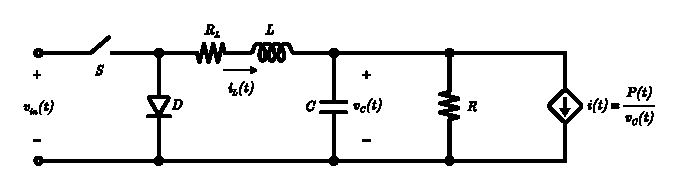
\includegraphics[scale=1.]{figures/buck_converter.eps}
  \caption{Buck converter circuit.}
  \label{fig:buck_converter}
\end{figure}

\subsection{Non-linear Buck Converter Model}

When the switch $S$ is in the off state fot the duration $t_{\rm{off}}$, the dynamic equations describing the circuit's behavior at this moment, derived from Kirchhoff's laws, are as follows:
\begin{equation}
  \begin{cases}
    \dot i_L = - \frac{R_L} L i(t) - \frac{1}{L} v_C(t) \\[8pt]
    \dot v_C = \frac{1}{C} i_L(t) - \frac{1}{C R} v_C(t) - \frac{1}{C v_C(t)} P_{\ell}(t)
  \end{cases}
  \label{eq:buck_state_off}
\end{equation}
And, when the switch $S$ is in the on state for the duration $t_{\rm{on}}$,
\begin{equation}
  \begin{cases}
    \dot i_L = - \frac{R_L} L i(t) - \frac{1}{L} v_C(t) + \frac{1}{L} v_{\rm{in}}(t) \\[8pt]
    \dot v_C = \frac{1}{C} i_L(t) - \frac{1}{C R} v_C(t) - \frac{1}{C v_C(t)} P_{\ell}(t)
  \end{cases}
  \label{eq:buck_state_on}
\end{equation}

Building on the equations \eqref{eq:buck_state_off} and \eqref{eq:buck_state_on}, the average dynamic model that represents the behavior of the buck converter throughout its operation is:
\begin{equation}
  \begin{cases}
    \dot i_L = \left[- \frac{R_L} L i(t) - \frac{1}{L} v_C(t) \right] \frac{t_{\rm{off}}}{t_{\rm{off}} + t_{\rm{on}}} + \left[- \frac{R_L} L i(t) - \frac{1}{L} v_C(t) + \frac{1}{L} v_{\rm{in}}(t)\right] \frac{t_{\rm{on}}}{t_{\rm{off}} + t_{\rm{on}}} \\[8pt]
    \dot v_C = \left[- \frac{1}{C} i_L(t) - \frac{1}{C R} v_C(t) - \frac{1}{C v_C(t)} P_{\ell}(t)\right] \frac{t_{\rm{off}}}{t_{\rm{off}} + t_{\rm{on}}} + \left[- \frac{1}{C} i_L(t) - \frac{1}{C R} v_C(t) - \frac{1}{C v_C(t)} P_{\ell}(t)\right] \frac{t_{\rm{on}}}{t_{\rm{off}} + t_{\rm{on}}}
  \end{cases}
  \label{eq:buck_average_model_1}
\end{equation}

Defining the following expression:
\begin{equation}
  d = \frac{t_{\rm{on}}}{t_{\rm{off}} + t_{\rm{on}}},
\end{equation}
yields,
\begin{equation}
  \frac{t_{\rm{off}} + t_{\rm{on}}}{t_{\rm{off}} + t_{\rm{on}}} = 1 \Rightarrow
  \frac{t_{\rm{off}}}{t_{\rm{off}} + t_{\rm{on}}}
  + \frac{t_{\rm{on}}}{t_{\rm{off}} + t_{\rm{on}}} = 1 \Rightarrow
  \frac{t_{\rm{off}}}{t_{\rm{off}} + t_{\rm{on}}} = 1 - \frac{t_{\rm{on}}}{t_{\rm{off}} + t_{\rm{on}}} \Rightarrow
  \frac{t_{\rm{off}}}{t_{\rm{off}} + t_{\rm{on}}} = 1 - d
\end{equation}

Therefore, the equation \eqref{eq:buck_average_model_1} can be rewritten as follows:
\begin{equation*}
  \begin{cases}
    \dot i_L = \left[- \frac{R_L} L i(t) - \frac{1}{L} v_C(t) \right] \left(1 - d\right) + \left[- \frac{R_L} L i(t) - \frac{1}{L} v_C(t) + \frac{1}{L} v_{\rm{in}}(t)\right] d \\[8pt]
    \dot v_C = \left[- \frac{1}{C} i_L(t) - \frac{1}{C R} v_C(t) - \frac{1}{C v_C(t)} P_{\ell}(t)\right] \left(1 - d\right) + \left[- \frac{1}{C} i_L(t) - \frac{1}{C R} v_C(t) - \frac{1}{C v_C(t)} P_{\ell}(t)\right] d
  \end{cases}
\end{equation*}
Then,
\begin{equation}
  \begin{cases}
    \dot i_L = - \frac{R_L} L i(t) - \frac{1}{L} v_C(t) + \frac{1}{L} v_{\rm{in}}(t) d \\[8pt]
    \dot v_C = - \frac{1}{C} i_L(t) - \frac{1}{C R} v_C(t) - \frac{1}{C v_C(t)} P_{\ell}(t)
  \end{cases}
  \label{eq:buck_conveter_nonlinear_model}
\end{equation}

The variable $d$ is commonly known as the switching duty cycle, which plays a crucial role in controlling switch states. Its value can be determined based on the control input $u_d(t)$, defined by:
\begin{equation}
  d(u_d(t)) = \max\left\{\min\{u_d(t), 1\}, 0\right\}.
\end{equation}
Choosing the operation point $P^{\rm o} = (i_L^{\rm o}, v_C^{\rm o}, u_d^{\rm o}, v_{\rm in}^{\rm o}, P_{\ell}^{\rm o})$, where $u_d^{\rm o} \in \left[0,1\right]$, the following coordinate change can be performed:
\begin{gather}
  \begin{align}
    \delta i_L(t) & = i_L(t) - i_L^{\rm o}, &
    \delta v_C(t) & = v_C(t) - v_C^{\rm o}, &
    \delta u_d(t) & = u_d(t) - u_d^{\rm o}
  \end{align} \\
  \begin{align}
    \delta v_{\rm in}(t) & = v_{\rm in}(t) - v_{\rm in}^{\rm o} &
    \delta P_{\ell}(t)   & = P_{\ell}(t) - P_{\ell}^{\rm o}
  \end{align}
\end{gather}
Moreover, let the control input saturation be modeled by means of the function $\rm{sat} : \mathbb{R} \rightarrow \left[-\upsilon , \upsilon  \right]$ such that:
\begin{gather}
  \delta d = {\rm sat} (\delta u_d(t)) = \max\left\{\min\left\{\delta u_d(t), \upsilon\right\}, -\upsilon\right\} \\
  \upsilon = \min\left\{1 - u_d^{\rm o}, u_d^{\rm o}\right\}
\end{gather}
Thus, the following non-linear model is obtained:
\begin{equation}
  \begin{cases}
    \delta \dot i_L = - \frac{R_L} L \delta i(t) - \frac{1}{L} \delta v_C(t) + \frac{v_{\rm{in}}^{\rm o} +\delta v_{\rm{in}}(t)}{L} {\rm sat}(\delta u_d(t)) + \frac{u_d^{\rm o}}{L} \delta v_{\rm in} (t) \\[8pt]
    \delta \dot v_C = \frac{1}{C} \delta i_L(t) + \left[- \frac{1}{C R}
      + \frac{P_{\ell}^o}{C v_C^o \left[v_C^o + \delta v_C(t)\right]} \right] \delta v_C(t)
    - \frac{1}{C \left[v_C^{\rm o} + \delta v_C(t)\right] } \delta P_{\ell}(t)
  \end{cases}
  \label{eq:buck_conveter_nonlinear_model_sat}
\end{equation}
where, 
\begin{align}
  & \begin{aligned}
      i_L^{\mathrm{o}} & = \frac{1}{R} v_C^{\mathrm{o}} + \frac{1}{v_C^{\mathrm{o}}} P_{\ell}^{\mathrm{o}},
    \end{aligned}
  & \begin{aligned}
      u_d^{\mathrm{o}} & = \frac{R_L}{v_{\mathrm{in}}^{\rm o}} i_L^{\mathrm{o}} + \frac{v_C^{\mathrm{o}}}{v_{\mathrm{in}}^{\rm o}}.
    \end{aligned}
    \notag
\end{align}
Finally, the model \eqref{eq:buck_conveter_nonlinear_model_sat} can be rewritten as:
\begin{equation}
  \dot x = A(x) x(t) + B(w) {\rm sat}(u(t)) + E(x,u) w(t)
  \label{eq:buck_conveter_nonlinear_model_ssm}
\end{equation}
where $x(t) = \begin{bmatrix}i_L(t) & v_C(t)\end{bmatrix}^{\rm{T}}$, $u(t) = \delta u_d(t)$, $w(t) = \begin{bmatrix} \delta v_{\rm in}(t) & \delta P_{\ell}(t)\end{bmatrix}^{\rm{T}}$, and
\begin{gather}
  \notag
  \begin{align}
    A(x) & = \begin{bmatrix}
               - \frac{R_L}{L} & - \frac{1}{L}                                                                   \\[8pt]
               \frac{1}{C}     & - \frac{1}{C R} + \frac{P_{\ell}^o}{C v_C^o \left[v_C^o + \delta v_C(t)\right]}
             \end{bmatrix} &
    B(w) & = \begin{bmatrix}
               \frac{v_{\rm{in}}^{\rm o} +\delta v_{\rm{in}}(t)}{L} \\[8pt] 0
             \end{bmatrix}
  \end{align}
  % \label{eq:buck_conveter_nonlinear_model_ssm_ab} 
  \\[12pt]
  E(x,u) = \begin{bmatrix}
    \frac{u_d^{\rm o}}{L} & 0 \\[8pt] 0 &  - \frac{1}{C \left[v_C^{\rm o} + \delta v_C(t)\right] }
  \end{bmatrix}
  \label{eq:buck_conveter_nonlinear_model_ssm_e}
\end{gather}

\subsection{Buck Converter Fuzzy Model}

In order to address the nonlinearity introduced by saturation, an approach based on substituting ${\rm sat(\circ)}$ with a dead-zone type nonlinearity is used. The dead-zone nonlinearity is defined as:
\begin{equation}
  \psi(u(t)) \triangleq u(t) - {\rm sat}(u(t))
\end{equation}
From the matrices presented in equation \eqref{eq:buck_conveter_nonlinear_model_ssm_e}, it follows $\frac{1}{v_C^{\rm o} + \delta v_C^{\rm o}}$ and $v_{\rm{in}}^{\rm o} +\delta v_{\rm{in}}(t)$ are non-linear terms. For the non-linear terms, are defined
\begin{align}
  z_0(t) & \equiv \frac{1}{v_C^{\rm o} + \delta v_C^{\rm o}}  & \txt{and} &  &
  z_1(t) & \equiv v_{\rm{in}}^{\rm o} +\delta v_{\rm{in}}(t).
\end{align}
Thus, the equation \eqref{eq:buck_conveter_nonlinear_model_ssm} can be rewritten as:
\begin{equation}
  \dot x = A(z(t)) x(t) + B(z(t)) u(t) - B(w) \psi(u(t)) + E(z(t)) w(t),
\end{equation}
where $z(t) = \begin{bmatrix}z_0(t) & z_1(t)\end{bmatrix}$, $A(z(t))  = \begin{bmatrix}
    - \frac{R_L}{L} & - \frac{1}{L}                                       \\[8pt]
    \frac{1}{C}     & - \frac{1}{C R} + \frac{P_{\ell}^o}{C v_C^o} z_0(t)
  \end{bmatrix}$, $B(z(t))  = \begin{bmatrix}
    \frac{1}{L} z_1(t) \\[8pt] 0
  \end{bmatrix}$ and $E(z(t))  = \begin{bmatrix}
    \frac{u_d^{\rm o}}{L} & 0 \\[8pt] 0   & - \frac{1}{C} z_0(t)
  \end{bmatrix}$.

Next, the minimum and maximum values of $z_0(t)$ e $z_1(t)$ under $v_C(t) \in \left[v_C^{\rm{min}}, v_C^{\rm{max}}\right]$ and $v_{\rm{in}}(t) \in \left[v_{\rm{in}}^{\rm{min}}, v_{\rm{in}}^{\rm{max}}\right]$, are obtained as follows:
\begin{equation}
  \begin{cases}
    z_i^0 & = \min\limits_{v_C(t), v_{\rm{in}}(t)} z_i(t) \\[8pt]
    z_i^1 & = \max\limits_{v_C(t), v_{\rm{in}}(t)} z_i(t)
  \end{cases}, \hspace{12pt }i = 1, 2
\end{equation}

From the maximum and minimum values of $z_0(t)$ and $z_1(t)$, the membership functions can be calculated as:
\begin{equation}
  z_i(t) = \sum\limits_{j = 0}^{1} M_i^{j}(z_i(t)) z_i^{j}, \hspace{12pt} \txt{where }
  \hspace{12pt} M_i^1 = \frac{z_i(t) - z_i^0}{z_i^1 - z_i^0} \hspace{8pt} \txt{and} \hspace{8pt}
  M_i^0 = 1 - M_i^1,
  \hspace{12pt} \txt{for} i = \{1,2\}.
\end{equation}

Therefore, the Takagi-Sugeno fuzzy model for the buck converter is:
\begin{equation}
  \dot x = \sum\limits_{i=0}^1 \sum\limits_{j=0}^1 \prod\limits_{k=1}^2 M_k^i(z_k(t))
  \left[
    A\left(z^{\left\{i,j\right\}}\right) x(t) +
    B\left(z^{\left\{i,j\right\}}\right) u(t) -
    B\left(z^{\left\{i,j\right\}}\right) \psi(u(t)) +
    E\left(z^{\left\{i,j\right\}}\right) w(t)
  \right]
  \label{eq:buck_converter_fuzzy_model_summations}
\end{equation}
where $z^{\left\{i,j\right\}}(t)$ is a shorthand for $\begin{bmatrix} z_1^i(t) & z_2^j(t) \end{bmatrix}$.

The summations in \eqref{eq:buck_converter_fuzzy_model_summations} can be aggregated as one summations:
\begin{equation}
  \dot x = \sum\limits_{p=\{0,0\}}^{\{1,1\}} h_p(z(t))
  \left\{A_p x(t) + B_p u(t) - B_p \psi(u(t)) + E_p w(t)\right\}
\end{equation}
where $p = \{b_1, b_2\} \in \mathbb{B}^2$, $\mathbb{B} = \{0,1\}$, 
\begin{gather}
  h_p(z(t)) = \prod\limits_{k=1}^2 M_k^{b_k} (z_k(t)) \\
  \begin{align}
    A_p &= A(z^p) & B_p &= B(z^p) & E_p &= E(z^p)
  \end{align}
\end{gather}

\chapter{Event-based Control for DC-DC Converters}

\section{Problem formulation}

Dynamic system:
\begin{equation}
  \dot x = \sum\limits_{p\in \mathbb{B}^n} h_p(z(t))
  \left\{A_p x(t) + B_p u(t) - B_p \psi(u(t)) + E_p w(t)\right\}
\end{equation}
\begin{gather}
  h_p(z(t)) = \prod\limits_{k=1}^n M_k^{b_k} (z_k(t)) \\
  \begin{align}
    A_p & = A(z^p) & B_p & = B(z^p) & E_p & = E(z^p)
  \end{align}
\end{gather}

Control law:
\begin{equation}
  u(t) = K(\hat x) \hat x(t) + L(\hat x) \hat w(t) \Rightarrow u(t) =  \sum\limits_{p\in \mathbb{B}^n} h_p(z(t))
  \left\{K_p \hat x(t)+ L_p \hat w(t)\right\}
\end{equation}

Consider a vector \( v \in \mathbb{R}^{n_u} \) such that the following set \(\mathcal{S}\) can be defined:
\begin{equation}
  \mathcal{S} = \left\{ u, v \in \mathbb{R}^{n_u} : |u_i - v_i| \leq {u_0}_i,\; i = 1, \dots, n_u \right\}
\end{equation}

If \( u \) and \( v \in \mathcal{S} \), then the relation
\begin{equation}
  \psi(u)^{\text{T}} T \left[\psi(u) - v\right] \leq 0
\end{equation}

is satisfied for any diagonal and positive definite matrix \( T \in \mathbb{R}^{n_u \times n_u} \).
\begin{equation}
  v = G(\hat x) x(t) = \sum\limits_{p\in \mathbb{B}^n} h_p(z(t))\left\{G_p \hat x(t)\right\}
\end{equation}
If $x \in \mathcal{S}$, such that
\begin{gather}
  \mathcal{S} = \left\{ x \in \mathbb{R}^{n} : | K(\hat x) \hat x(t) + L(\hat x) \hat w(t) - G(\hat x) \hat x(t)| \leq {u_0}_i,\; i = 1, \dots, n_u \right\} \\
  \mathcal{S} = \left\{ x \in \mathbb{R}^{n} : | \left[K(\hat x) - G(\hat x)\right] \hat x(t) + L(\hat x) \hat w(t)| \leq {u_0}_i,\; i = 1, \dots, n_u \right\} \\
  \mathcal{S} = \left\{ x \in \mathbb{R}^{n} : \left| \sum\limits_{p\in \mathbb{B}^n} h_p(z(t))\left\{(K_p - G_p) \hat x(t) + L_p \hat w(t) \right\}\right| \leq {u_0}_i,\; i = 1, \dots, n_u \right\}
\end{gather}
then,
\begin{equation}
  \psi^\text{T}(K(\hat x) x(t) + L(\hat x) \hat w) T\left[\psi(K(\hat x) \hat x + L(\hat x) \hat w) - G(\hat x) \hat x\right] \leq 0
\end{equation}

\begin{equation}
  \psi^\text{T}(u(t)) T\left[\psi(u(t)) - G(\hat x) \hat x\right] \leq 0
\end{equation}

\begin{equation}
  \psi^\text{T}(u(t)) T \psi(u(t)) - \psi^\text{T}(u(t)) T G(x(t) + e_x(t)) \left[x(t) + e_x(t)\right] \leq 0
\end{equation}

\begin{multline}
  \psi^\text{T}(u(t)) T \psi(u(t)) - \psi^\text{T}(u(t)) T G(x(t)) x(t) - \psi^\text{T}(u(t)) T G(x(t)) e_x(t) \\- \psi^\text{T}(u(t)) T G(e_x(t)) x(t) - \psi^\text{T}(u(t)) T G(e_x(t)) e_x(t)\leq 0
\end{multline}

\begin{multline}
  \psi^\text{T}(u(t)) T \psi(u(t)) - \psi^\text{T}(u(t)) T G(x(t)) x(t) - \psi^\text{T}(u(t)) T G(x(t)) e_x(t) \\- \psi^\text{T}(u(t)) T \left[G(x(t) + e_x(t)) - G(x)\right] \left[x(t) + e_x(t)\right]\leq 0
\end{multline}

\begin{equation}
  \psi^\text{T}(u(t)) T \psi(u(t)) - \psi^\text{T}(u(t)) T G(x(t)) x(t) - \psi^\text{T}(u(t)) T G(x(t)) e_x(t) - \psi^\text{T}(u(t)) TG(e_x(t)) \left[x(t) + e_x(t)\right] \leq 0
\end{equation}

\subsection{Sistema}

Seja $e_x(t) = \hat x(t) - x(t)$ and $e_w(t) = \hat w(t) - w(t)$. Têm-se,
\begin{gather}
  \dot x = A(x) x(t) + B(x) u(t) - B \psi(u(t)) + E(x) w(t) \\
  \dot x = A(x) x(t) + B(x) \left[K(\hat x) \hat x(t) + L(\hat x) \hat w(t)\right] - B \psi(u(t)) + E(x) w(t) \\
  \dot x = A(x) x(t) + B(x) K(\hat x) \hat x(t) + B(x) L(\hat x) \hat w(t) - B \psi(u(t)) + E(x) w(t)
\end{gather}
\begin{multline}
  \dot x = A(x) x(t) + B(x) K(\hat x(t)) \left[e_x(t) + x(t)\right] \\ + B(x) L(\hat x(t)) \left[e_w(t) + w(t)\right] - B \psi(u(t)) + E(x) w(t)
\end{multline}
\begin{multline}
  \dot x = \left[A(x) + B(x) K(x(t)) \right] x(t) + B(x) K(x(t)) e_x(t) + B(x) K(e_x(t)) \left[e_x(t) + x(t)\right] \\ + \left[E(x) + B(x) L(x(t)) \right] w(t) + B(x) L(x(t)) e_w(t) + B(x) L(e_x(t)) \left[e_w(t) + w(t)\right] \\ - B \psi(u(t))
\end{multline}

ETM dinâmico:
\begin{equation}
  t_0 = 0, t_{k+1} = \inf \{t > t_k : \eta(t) + \theta \Gamma(x(t), e_x(t), e_w(t)) < 0 \}, \, \forall k \in \mathbb{N}.
\end{equation}
Função de ativação:
\begin{equation}
  \Gamma(x, e_x) = x^T(t) \Psi x(t) - e_x^T \Xi_x e_x - \zeta(x, e_x)
\end{equation}
onde,
\begin{equation}
  \zeta(x, e_x) = 2 x^T P\left[B(x) \left(K(x+e_x) - x\right)(x+e_x)\right]
\end{equation}

LMI de restrição,
\begin{equation}
  \begin{bmatrix}
    \txt{\bf He}(A_i X + B_i \tilde K_j) + (1 - \beta) I & E_i X + B_i \tilde L_j & B_i \tilde K_j      & B_i \tilde L_j & -B_i X - \frac{1}{2} X TG_i X & X             \\
    \star                                         & -(\mu - \alpha)I          & 0                   & 0              & 0                             & 0             \\
    \star                                         & \star                     & -\tilde \Xi - \beta & 0              & -\frac{1}{2}XTG_iX           & 0             \\
    \star                                         & \star                     & \star               & \alpha I       & 0                             & 0             \\
    \star                                         & \star                     & \star               & \star          & \tilde T                      & 0             \\
    \star                                         & \star                     & \star               & \star          & \star                         & - \tilde \Psi \\
  \end{bmatrix} < 0
\end{equation}

Multiplicando por $diag(X^{-1}, X^{-1}, X^{-1}, X^{-1}, I)$, e fazendo as mudança de variáveis: $K_j = \tilde{K_j} X^{-1}$, $L_j = \tilde{L_j} X^{-1}$, $\Xi = X^{-1} \tilde \Xi X^{-1}$, $T = X^{-1} \tilde T X^{-1}$, $P =  X^{-1}$

\begin{equation}
  \begin{bmatrix}
    \Omega & P \left[E(x) + B(x)L(x)\right] & PB(x)K(x)    & PB(x)L(x) & -PB(x) - \frac{1}{2}TG(x) & I             \\
    \star  & -(\mu - \alpha)I               & 0            & 0         & 0                         & 0             \\
    \star  & \star                          & -\Xi - \beta & 0         & -\frac{1}{2}TG(x)         & 0             \\
    \star  & \star                          & \star        & \alpha I  & 0                         & 0             \\
    \star  & \star                          & \star        & \star     & T                         & 0             \\
    \star  & \star                          & \star        & \star     & \star                     & - \tilde \Psi \\
  \end{bmatrix} < 0
\end{equation}

onde $\Omega = P \txt{\bf He}(A(x) + B(x)K(x)) + (1 - \beta) I$. Pelo complemento de Schur,
\begin{equation}
  \begin{bmatrix}
    \Omega + \Psi & P \left[E(x) + B(x)L(x)\right] & PB(x)K(x)    & PB(x)L(x) & -PB(x) - \frac{1}{2}TG(x) \\
    \star         & -(\mu - \alpha)I               & 0            & 0         & 0                         \\
    \star         & \star                          & -\Xi - \beta & 0         & -\frac{1}{2}TG(x)         \\
    \star         & \star                          & \star        & \alpha I  & 0                         \\
    \star         & \star                          & \star        & \star     & T
  \end{bmatrix} < 0
\end{equation}

Considerando $v = \begin{bmatrix} x^T(t) & w^T(t) & e_x^T(t) & e_w^T(t) & \psi(u)^T \end{bmatrix}$, pré e pós-multiplicando por $v$ e $v^T$, respectivamente, obtêm-se:
\begin{multline}
  2x^T(t)P\left\{\left[A(x) + B(x) K(x(t)) \right] x(t) + \left[E(x) + B(x) L(x(t)) \right] w(t)  + B(x) K(x(t)) e_x(t) + B(x) L(x(t)) e_w(t)  \right.
  \\ \left. - B(x) \psi(u(t))\right\} - \psi^T(u(t))TG(x)x(t) + (1 - \beta) x^T(t)x(t) - (\mu - \alpha) w^T(t) w(t) + x^T(t) \Psi x(t) - e_x^T(t) \Xi e_x(t)
  \\ - \beta e^T_x(t) e_x(t)+ \alpha e_w^T(t)e_w(t) + \psi^T(u(t))T\psi(u(t)) - \psi^T(u(t)) TG(x) e_x(t)< 0
\end{multline}

Onde $\alpha \in \mathbb{R}_{>0}$ é tal que:
\begin{equation}
  2x^TPB(x)L(e_x(t)) \left[w(t) + e_w(t)\right] \leq \alpha^{-1} \|x^T(t)PB(x)L(e_x)\|^2 + \alpha \|w(t) + e_w(t)\|^2
\end{equation}
\begin{equation}
  2x^TPB(x)L(e_x(t)) \left[w(t) + e_w(t)\right] \leq \alpha^{-1} \|x^T(t)PB(x)L(e_x)\|^2 + \alpha \|w(t)\|^2 + \alpha \|w(t)\| \|e_w(t)\|+ \alpha\|e_w(t)\|^2
\end{equation}
\begin{equation}
  - \alpha^{-1} \|x^T(t)PB(x)L(e_x)\|^2 - \alpha \|w(t)\|^2 - \alpha \|w(t)\| \|e_w(t)\| - \alpha\|e_w(t)\|^2 \leq - 2x^TPB(x)L(e_x(t)) \left[w(t) + e_w(t)\right]
\end{equation}

Assim,
\begin{multline}
  2x^T(t)P\left\{\left[A(x) + B(x) K(x(t)) \right] x(t) + \left[E(x) + B(x) L(x(t)) \right] w(t)  + B(x) K(x(t)) e_x(t) + B(x) L(x(t)) e_w(t)  \right.
  \\ \left. - B(x) \psi(u(t))\right\} - \psi^T(u(t))TG(x)x(t) + (1 - \beta) x^T(t)x(t) - \mu w^T(t) w(t) + x^T(t) \Psi x(t) - e_x^T(t) \Xi e_x(t) - \beta e^T_x(t) e_x(t)
  \\  + \psi^T(u(t))T\psi(u(t)) - \psi^T(u(t)) TG(x) e_x(t) < - \alpha w^T(t) w(t) - \alpha e_w^T(t)e_w(t)
\end{multline}
\begin{multline}
  2x^T(t)P\left\{\left[A(x) + B(x) K(x(t)) \right] x(t) + \left[E(x) + B(x) L(x(t)) \right] w(t)  + B(x) K(x(t)) e_x(t) + B(x) L(x(t)) e_w(t)  \right.
  \\ \left. - B(x) \psi(u(t))\right\} - \psi^T(u(t))TG(x)x(t) + (1 - \beta) x^T(t)x(t) - \mu w^T(t) w(t) + x^T(t) \Psi x(t) - e_x^T(t) \Xi e_x(t) - \beta e^T_x(t) e_x(t)
  \\ + \psi^T(u(t))T\psi(u(t)) - \psi^T(u(t)) TG(x) e_x(t)  - \alpha \|w(t)\| \|e_w(t)\| - \alpha^{-1} \|x^T(t)PB(x)L(e_x)\|^2
  \\ < - \alpha w^T(t) w(t) - \alpha e_w^T(t)e_w(t)  - \alpha \|w(t)\| \|e_w(t)\| - \alpha^{-1} \|x^T(t)PB(x)L(e_x)\|^2
\end{multline}
\begin{multline}
  2x^T(t)P\left\{\left[A(x) + B(x) K(x(t)) \right] x(t) + \left[E(x) + B(x) L(x(t)) \right] w(t)  + B(x) K(x(t)) e_x(t) + B(x) L(x(t)) e_w(t)  \right.
  \\ \left. - B(x) \psi(u(t))\right\} - \psi^T(u(t))TG(x)x(t) + (1 - \beta) x^T(t)x(t) - \mu w^T(t) w(t) + x^T(t) \Psi x(t) - e_x^T(t) \Xi e_x(t) - \beta e^T_x(t) e_x(t)
  \\ + \psi^T(u(t))T\psi(u(t)) - \psi^T(u(t)) TG(x) e_x(t)  - \alpha \|w(t)\| \|e_w(t)\| - \alpha^{-1} \|x^T(t)PB(x)L(e_x)\|^2
  \\ < - 2x^TPB(x)L(e_x(t)) \left[w(t) + e_w(t)\right]
\end{multline}
\begin{multline}
  2x^T(t)P\left\{\left[A(x) + B(x) K(x(t)) \right] x(t) + \left[E(x) + B(x) L(x(t)) \right] w(t)  + B(x) K(x(t)) e_x(t) + B(x) L(x(t)) e_w(t)  \right.
  \\ \left. + B(x)L(e_x(t)) \left[w(t) + e_w(t)\right] - B(x) \psi(u(t))\right\} - \psi^T(u(t))TG(x)x(t) + (1 - \beta) x^T(t)x(t) - \mu w^T(t) w(t) \\ + x^T(t) \Psi x(t) - e_x^T(t) \Xi e_x(t) - \beta e^T_x(t) e_x(t) + \psi^T(u(t))T\psi(u(t)) - \psi^T(u(t)) TG(x) e_x(t)  - \alpha \|w(t)\| \|e_w(t)\| \\ - \alpha^{-1} \|x^T(t)PB(x)L(e_x)\|^2  < 0
\end{multline}
\begin{multline}
  2x^T(t)P\left\{\left[A(x) + B(x) K(x(t)) \right] x(t) + \left[E(x) + B(x) L(x(t)) \right] w(t)  + B(x) K(x(t)) e_x(t) + B(x) L(x(t)) e_w(t)  \right.
  \\ \left. + B(x)L(e_x(t)) \left[w(t) + e_w(t)\right] - B(x) \psi(u(t))\right\} - \psi^T(u(t))TG(x)x(t) + (1 - \beta) x^T(t)x(t) - \mu w^T(t) w(t) \\ + x^T(t) \Psi x(t) - e_x^T(t) \Xi e_x(t) - \beta e^T_x(t) e_x(t) + \psi^T(u(t))T\psi(u(t)) - \psi^T(u(t)) TG(x) e_x(t)  < 0
\end{multline}
Somando $\zeta(x(t), e_x(t))$, têm-se:
\begin{multline}
  2x^T(t)P\dot x(t) - \psi^T(u(t))TG(x)x(t) + (1 - \beta) x^T(t)x(t) - \mu w^T(t) w(t) \\ + x^T(t) \Psi x(t) - e_x^T(t) \Xi e_x(t) - \beta e^T_x(t) e_x(t) + \psi^T(u(t))T\psi(u(t)) - \psi^T(u(t)) TG(x) e_x(t)  < 0
\end{multline}

De forma semelhante, $\beta \in \mathbb{R}_{>0}$ é tal que,
\begin{equation}
  \psi^T(u(t))G(e_x(t)) \left[x(t) + e_x(t)\right] \leq \beta^{-1} \|\psi(u(t))G(e_x(t))\|^2 + \beta \|x(t) + e_x(t)\|^2
\end{equation}
\begin{equation}
  \psi^T(u(t))G(e_x(t)) \left[x(t) + e_x(t)\right] - \beta^{-1} \|\psi(u(t))G(e_x(t))\|^2 - \beta \|x(t)\|^2 - \beta \|x(t)\|\|e_x(t)\| - \beta \|e_x(t)\|^2 \leq 0
\end{equation}

Logo,
\begin{multline}
  2x^T(t)P\dot x(t) + x^T(t)x(t) - \mu w^T(t) w(t) + x^T(t) \Psi x(t) - e_x^T(t) \Xi e_x(t) - \beta x^T(t) x(t)  + \psi^T(u(t))T\psi(u(t))  \\ - \psi^T(u(t))TG(x)x(t) - \psi^T(u(t)) TG(x) e_x(t) - \psi^T(u(t))G(e_x(t)) \left[x(t) + e_x(t)\right]  \\
  + \psi^T(u(t))G(e_x(t)) \left[x(t) + e_x(t)\right] - \beta e^T_x(t) e_x(t) < 0
\end{multline}

De, , % referir a equação com da saturação
\begin{multline}
  2x^T(t)P\dot x(t) + x^T(t)x(t) - \mu w^T(t) w(t) + x^T(t) \Psi x(t) - e_x^T(t) \Xi e_x(t) \\
  + \psi^T(u(t))G(e_x(t)) \left[x(t) + e_x(t)\right]  - \beta x^T(t) x(t) - \beta e^T_x(t) e_x(t) < 0
\end{multline}
\begin{multline}
  2x^T(t)P\dot x(t) + x^T(t)x(t) - \mu w^T(t) w(t) + x^T(t) \Psi x(t) - e_x^T(t) \Xi e_x(t)
  + \psi^T(u(t))G(e_x(t)) \left[x(t) + e_x(t)\right]  \\ - \beta x^T(t) x(t) - \beta e^T_x(t) e_x(t)  - \beta \|x(t)\|\|e_x(t)\| - \beta^{-1} \|\psi(u(t))G(e_x(t))\|^2  < 0
\end{multline}
\begin{equation}
  2x^T(t)P\dot x(t) + x^T(t)x(t) - \mu w^T(t) w(t) + x^T(t) \Psi x(t) - e_x^T(t) \Xi e_x(t) < 0
\end{equation}

Como $\lambda \eta(t) > 0$, então:
\begin{equation}
  2x^T(t)P\dot x(t) + x^T(t)x(t) - \mu w^T(t) w(t) + x^T(t) \Psi x(t) - e_x^T(t) \Xi e_x(t) - \lambda \eta(t) < 0
\end{equation}

Logo,
\begin{equation}
  \dot x^T(t)Px(t) + x^T(t)P\dot x(t) + \dot \eta(t) + x^T(t)x(t) - \mu w^T(t)w(t) < 0
\end{equation}
\begin{equation}
  \dot x^T(t)Px(t) + x^T(t)P\dot x(t) + \dot \eta(t) < 0
\end{equation}
\begin{equation}
  \dot W(x, \eta) < 0
\end{equation}

Portanto, a origem do sistema em malha fechada sob o ETM dinâmico é estável.

\end{document}
